\documentclass{article}
\usepackage[utf8]{inputenc}
\usepackage[italian]{babel}
\usepackage{amsmath}
\usepackage{amssymb}
\usepackage{siunitx}
\usepackage{tabularray}
\usepackage{graphicx}
\usepackage{float}
\usepackage{xfrac}
\newcommand*{\diam}{\varnothing}
\newcommand*{\best}[1]{{#1}_\text{best}}
\newcommand*{\bestp}[1]{{\left(#1\right)}_\text{best}}
\newcommand*{\pbest}[1]{\left({#1}_\text{best}\right)}
\newcommand*{\pbestp}[1]{\left({\left(#1\right)}_\text{best}\right)}
\newcommand*{\errrel}[1]{\frac{\delta #1}{{#1}_\text{best}}}
%% <custom footnotes/>
%\newcounter{savefootnote}
%\newcounter{symfootnote}
%\newcommand{\symfootnote}[1]{%
%   \setcounter{savefootnote}{\value{footnote}}%
%   \setcounter{footnote}{\value{symfootnote}}%
%   \ifnum\value{footnote}>8\setcounter{footnote}{0}\fi%
%   \let\oldthefootnote=\thefootnote%
%   \renewcommand{\thefootnote}{\fnsymbol{footnote}}%
%   \footnote{#1}%
%   \let\thefootnote=\oldthefootnote%
%   \setcounter{symfootnote}{\value{footnote}}%
%   \setcounter{footnote}{\value{savefootnote}}%
%}
%% </custom footnotes>
\title{
    Laboratorio di Fisica 1\\
    R8: Misura di $\left|\vec{g}\right|$ mediante rotolamento puro
}
\author{Gruppo 17: Bergamaschi Riccardo, Graiani Elia, Moglia Simone}
\date{19/03/2024 – 9/04/2024}
\makeindex
\begin{document}

\maketitle

\begin{abstract}
    Il gruppo di lavoro ha misurato indirettamente il modulo del campo gravitazionale locale ($g$)
    studiando il moto di rotolamento di un corpo rigido.

\setcounter{section}{-1}  % Count sections starting from 0
\section{Materiali e strumenti di misura utilizzati}
\begin{center}
    \begin{tblr}{ |Q[l,m]|Q[c,m]|Q[c,m]|Q[c,m]| }
        \hline
        \textbf{Strumento di misura} & \textbf{\:\:\:\:\:Soglia\:\:\:\:\:} & \textbf{Portata} & \textbf{Sensibilità} \\
        \hline
        {Due fototraguardi con \\ contatore di impulsi} & \qty{1}{\micro s} & \qty{99999999}{\micro s} & \qty{1}{\micro s} \\
        \hline[dashed]
        Metro a nastro & \qty{0.1}{cm} & \qty{300.0}{cm} & \qty{0.1}{cm} \\
        \hline[dashed]
        Calibro ventesimale & \qty{0.05}{mm} & \qty{150.00}{mm} & \qty{0.05}{mm} \\
        \hline[dashed]
        Bilancia di precisione & \qty{0.01}{g} & \qty{4200.00}{g} & \qty{0.01}{g} \\
        \hline
        \hline
        \textbf{Altro} & \SetCell[c=3]{l} \textbf{Descrizione/Note} \\
        \hline
        Brugola & \SetCell[c=3]{l} {
            Utile per cambiare la distanza \\
            tra i fototraguardi
        } \\
        \hline[dashed]
        Cellulare & \SetCell[c=3]{1} {
            Necessario per rilevare \\
            l'angolo di inclinazione
        } \\
        Un campione & \SetCell[c=3]{l} {Corpo rigido e simmetrico} \\
        \hline
    \end{tblr}
\end{center}

\section{Esperienza e procedimento di misura}
\begin{enumerate}
    \item
        Pesiamo il corpo con la bilancia di precisione per ottenerne la massa.
    \item
        Considerando il campione come una composizione di forme solide note
        di cui misuriamo tutti i diametri e le altezze necessarie al calcolo
        del suo momento d'inerzia con il calibro ventesimale.
    \item
        Acceso e impostato adeguatamente il contatore di impulsi,
        misuriamo 50 volte il tempo di caduta del campione
        variando l'angolo e le distanze tra i fototraguardi.
        
\end{enumerate}

\emph{
    \textbf{Notazione.} Indicheremo con $\left(t_s\right)_i$
    ogni $i$-esima misura del tempo di caduta
    $\left(i\in\left[0;50\right)\cap\mathbb{N}\right)$,
    mentre con $\overline{t_s}$ il tempo di caduta medio.
    In particolare:\[
        \delta\!\left(\overline{t_s}\right) = \sigma_{\overline{t_s}} =
        \frac{\sigma_{t_s}}{\sqrt{100}}   = \frac{\sigma_{t_s}}{10}.
    \]
}

\subsection{Analisi dei dati raccolti e conclusioni}
Fissato un sistema di riferimento solidale all'apparato di misura, con origine
nel punto di partenza del campione, possiamo
scrivere la seguente legge del moto:
\[x(t) = \frac{1}{2}g t^2\]
La norma di $\vec{g}$ misurata indirettamente è allora ricavabile da:
\begin{equation}\label{eq:1}
    g_s = \frac{2d_0 - \diam_i}{\left(\overline{t_s}\right)^2}
    % \best{g} = \frac{2\best{\left(d_0\right)} - \bestp{\diam_i}}
    %                 {\bestp{\overline{t_i}}^2}
    % \qquad\wedge\qquad
    % \errrel{g} = \frac{2\left(\delta d_0\right) - \delta \diam_i}
    %                   {2\best{\left(d_0\right)} - \bestp{\diam_i}}
    %            + 2\frac{\sigma_{\overline{t_i}}}{\overline{t_i}}
\end{equation}
dove l'errore su $g_s$ segue dalla propagazione degli errori su $d_0,\diam_s$ e
$\overline{t_s}$ (supponendo gli errori piccoli, casuali e indipendenti).

Di seguito riportiamo gli istogrammi dei tempi e i valori di $g$ così ottenuti.
Per confrontare queste misure indirette ($g_A$ e $g_B$) con il valore atteso
($g_\text{attesa}=\qty{9.806}{m\per s^2}$), valutiamo, per ogni sferetta $s$, la seguente quantità
(adimensionale):\[\varepsilon_s = \frac{\bestp{g_s} - g_\text{attesa}}{\delta g_s}
\] Allora la misura $g_s$ da noi ottenuta è compatibile con $g_\text{attesa}$ se e solo se
$\left|\varepsilon_s\right|\le1$; inoltre, dal segno di $\varepsilon_s$ è possibile
determinare se $g_s$ misurata è una sovrastima ($\varepsilon_s>0$) o una sottostima
($\varepsilon_s<0$) del valore atteso.

\begin{figure}[H]
    % trim={< v > ^}
    %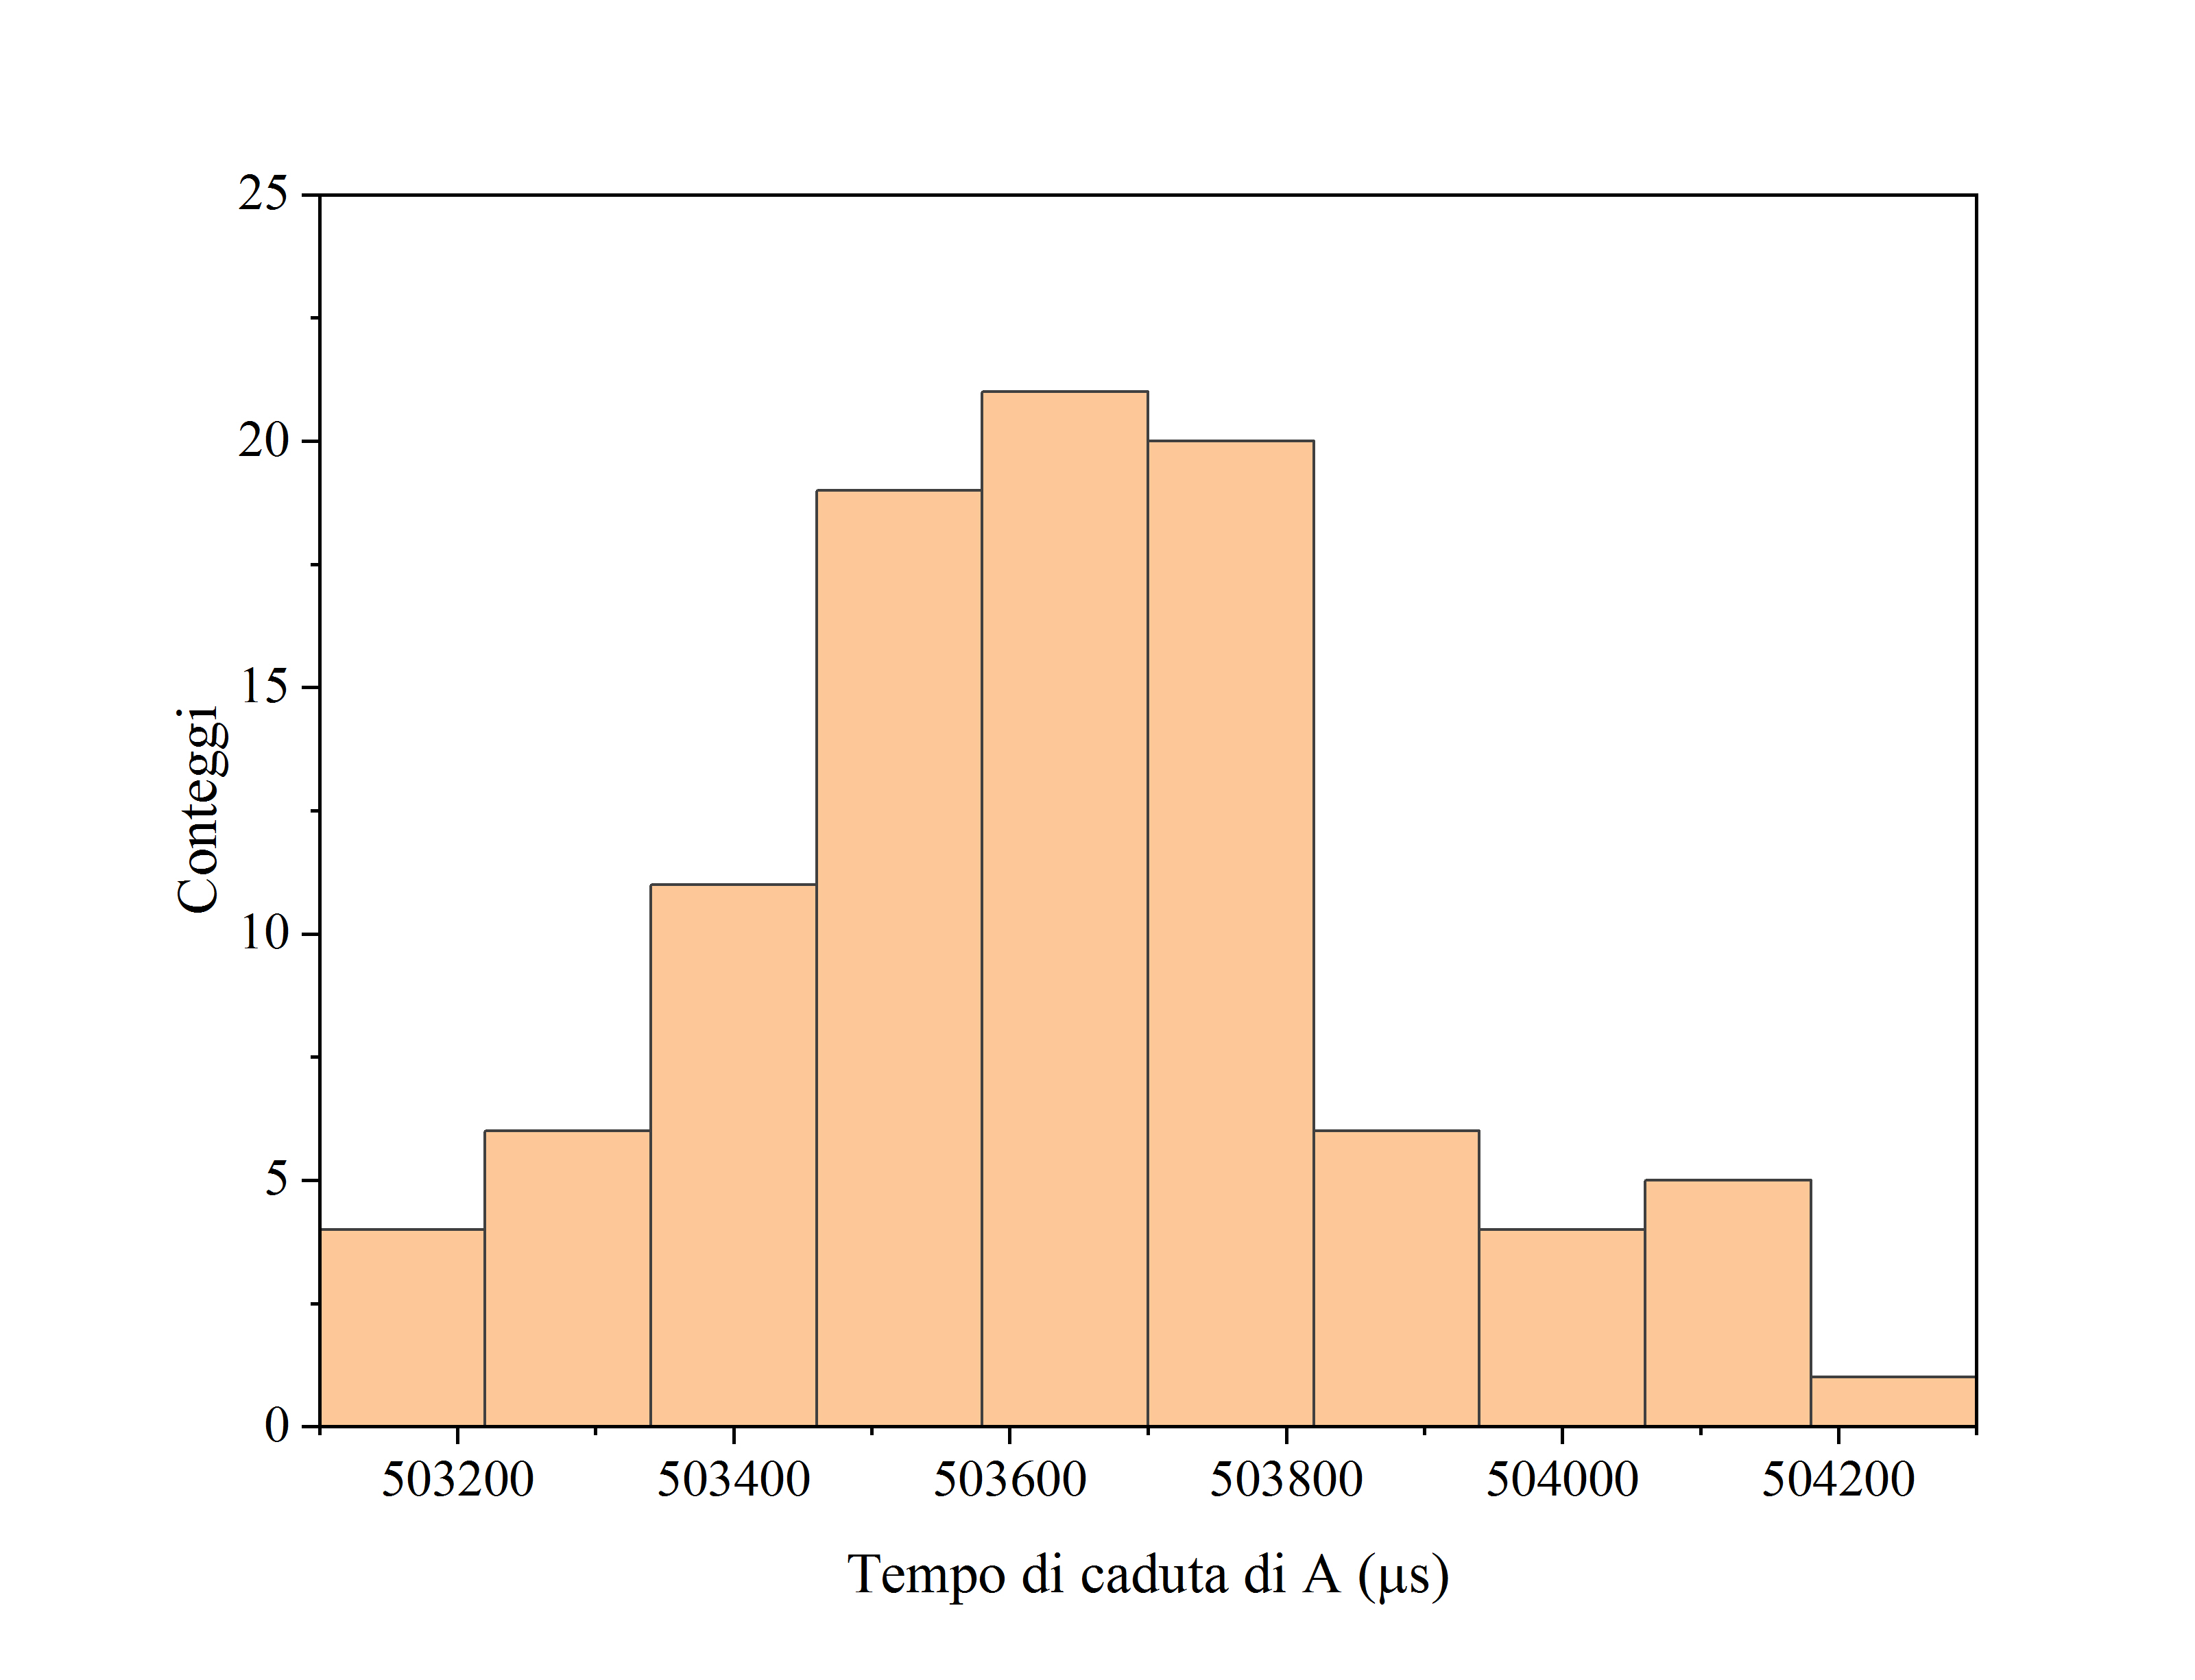
\includegraphics[trim={2cm .5cm 2.4cm 2.1cm},clip,width=.5\textwidth]{img/TempiA.jpg}
    %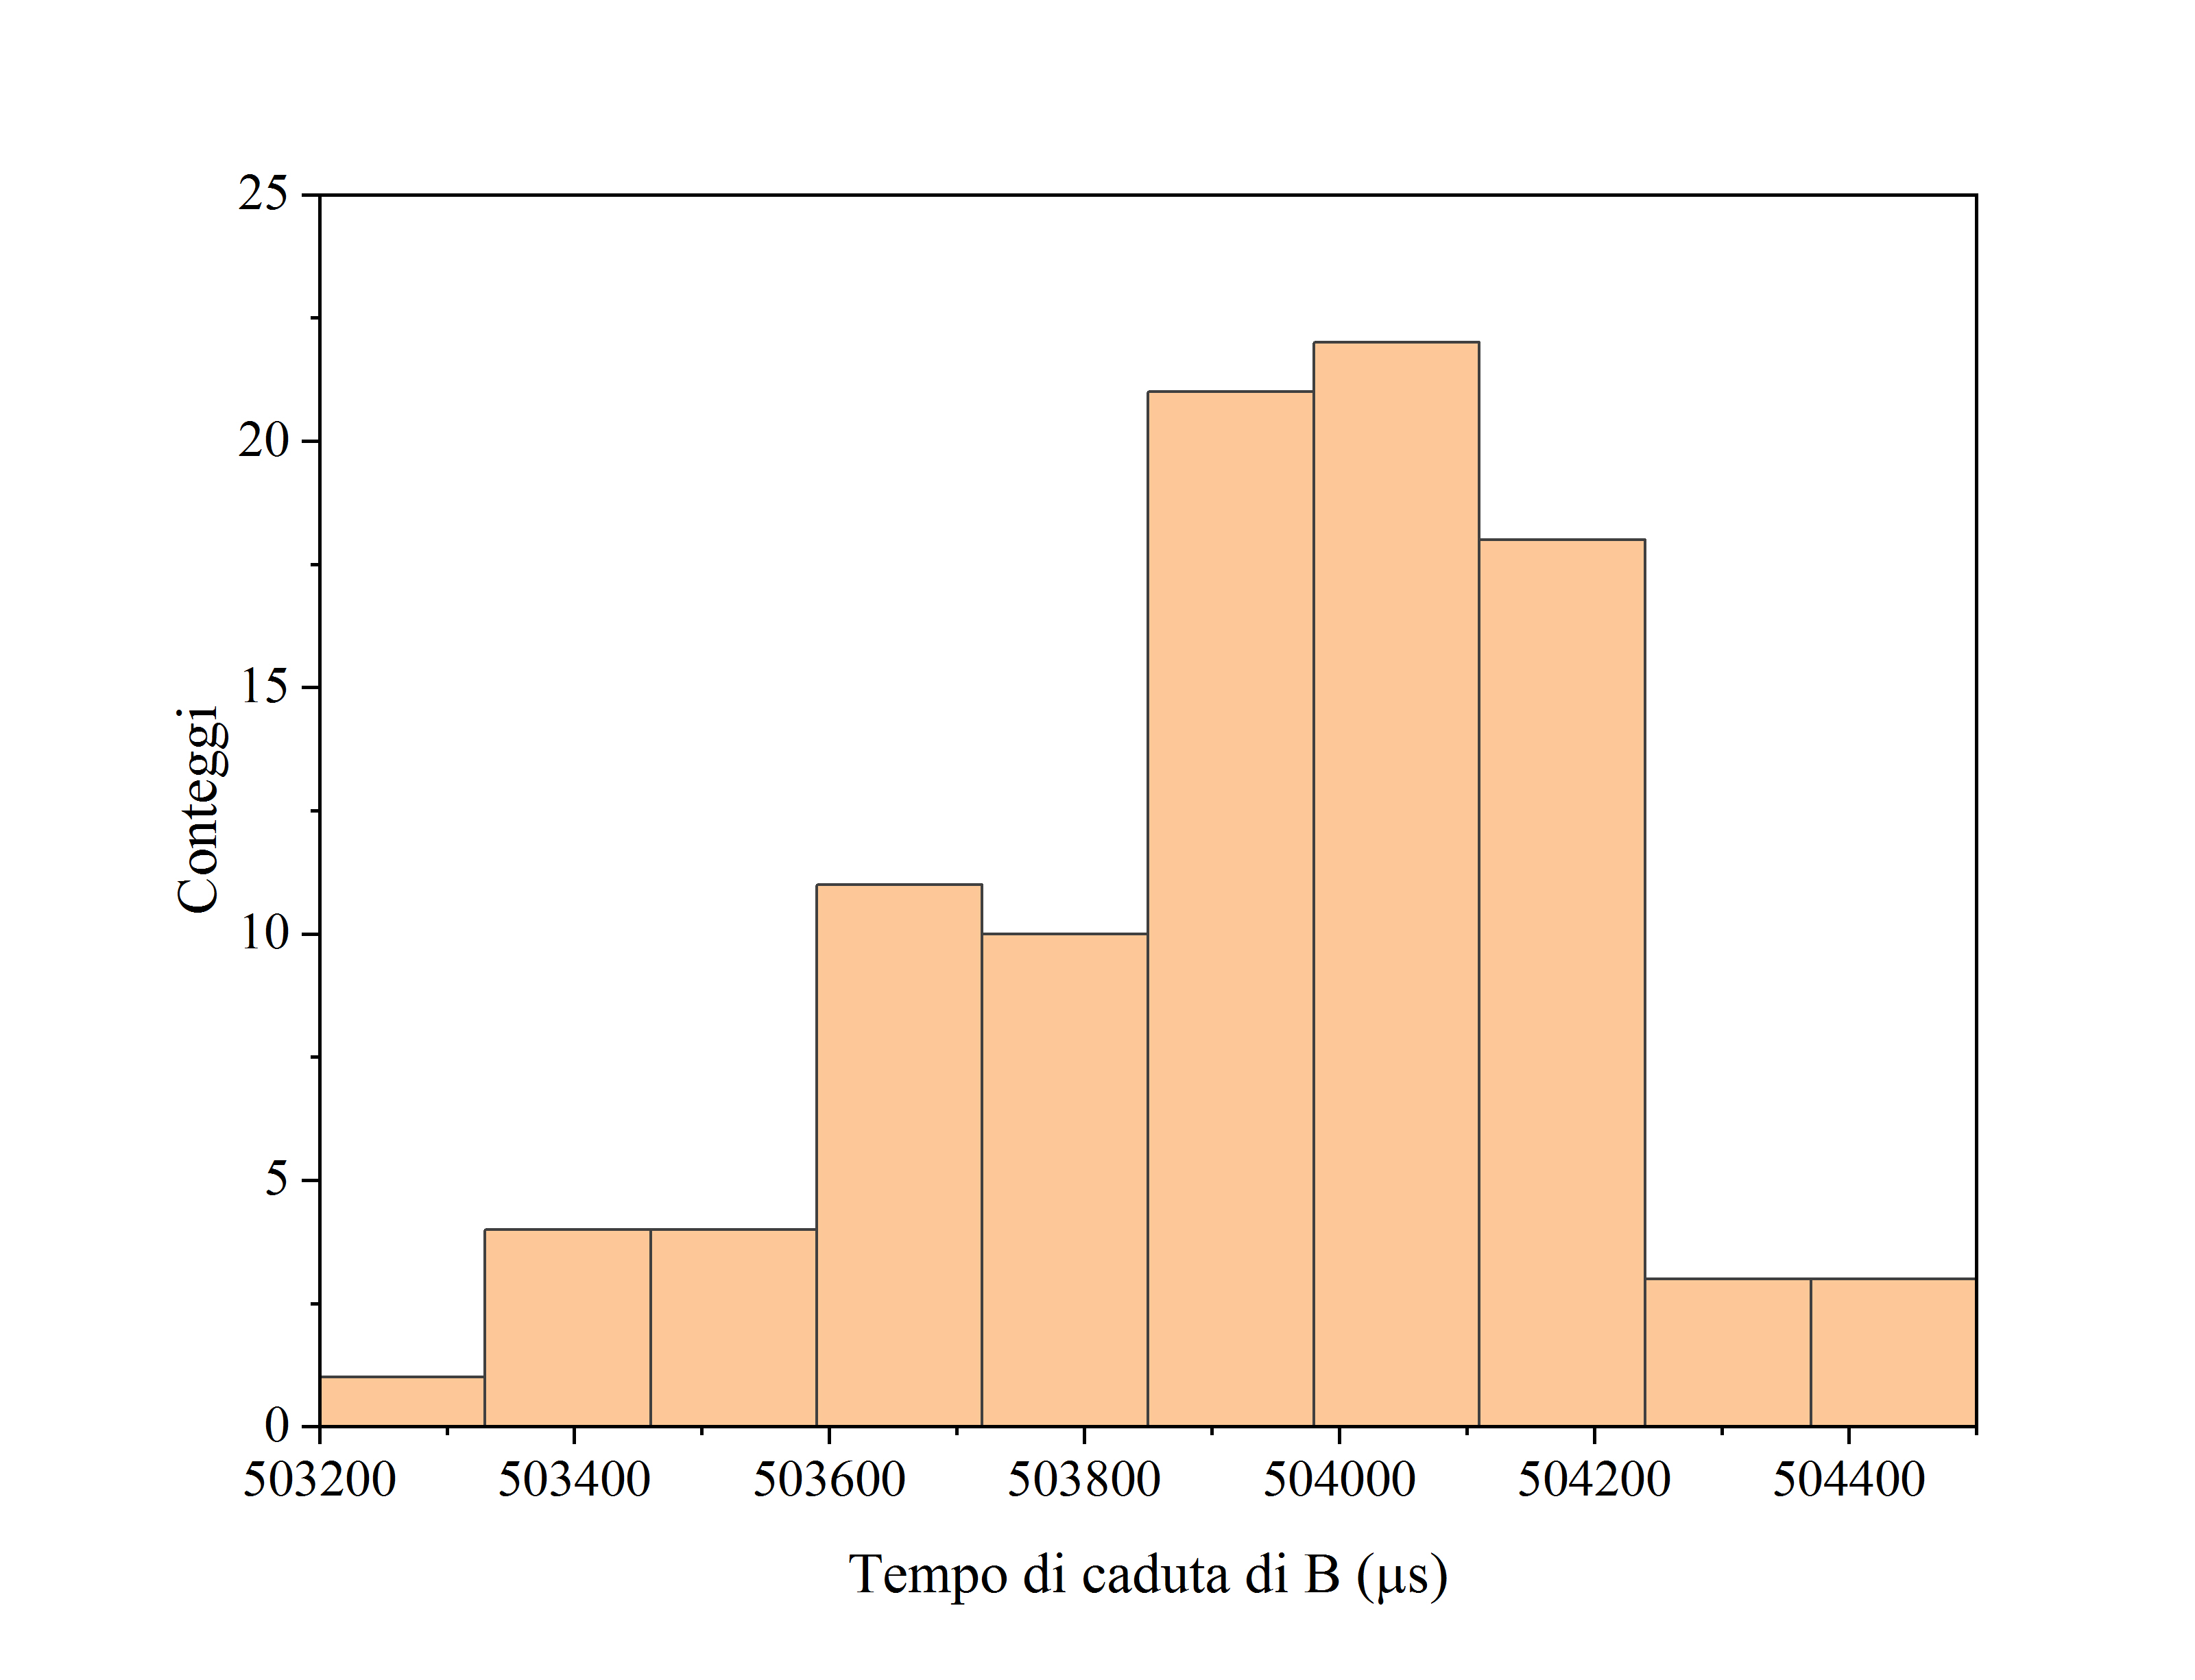
\includegraphics[trim={2cm .5cm 2.4cm 2.1cm},clip,width=.5\textwidth]{img/TempiB.jpg}
    \caption{Istogrammi dei dati raccolti ($t_A$ e $t_B$)}
\end{figure}
\vspace{.5cm}
\begin{center}
    \begin{tblr}{ |Q[c,m]|Q[c,m]|Q[c,m]|Q[c,m]|Q[c,m]| }
        \hline
            $s$ &
            $\diam_s\:(\unit{mm})$ &
            $\overline{t_s}\:(\unit{ms})$ &
            $g_s\:(\unit{m\per s^2})$ &
            $\varepsilon_s$ \\
        \hline
        A & $24.62\pm0.01$ & $503.63\pm0.02$ & $9.82\pm0.02$ & $+0.67$ \\
        \hline[dashed]
        B & $22.23\pm0.01$ & $503.93\pm0.02$ & $9.82\pm0.02$ & $+0.57$ \\
        \hline
    \end{tblr}
\end{center}

Le misure di $g$ ottenute sono pertanto ampiamente consistenti con il valore atteso.

\emph{
    \textbf{Osservazione.} Dai valori di $\varepsilon$ non emerge una differenza
    significativa fra le due sferette. In particolare, sembra che l'attrito viscoso
    dell'aria abbia agito in maniera trascurabile (come ci aspettavamo).\\
    Tuttavia, dopo una più attenta analisi, è comunque possibile notare una tendenza:
    in media, la sferetta con raggio maggiore ha percorso la stessa distanza in un
    tempo leggermente minore.
    Pertanto, ciò potrebbe suggerire un effetto molto ridotto dell'attrito dell'aria;
    questa tendenza però non è rispecchiata dai valore di $\varepsilon$,
    probabilmente a causa di una sovrastima della distanza $d_0$. Si noti infatti che,
    dal segno degli $\varepsilon$, entrambe le misure di $g$ sono risultate sovrastime,
    mentre, nell'equazione (\ref{eq:1}), $d_0$ è al numeratore.
}
\end{document}
